\chapter{绪论}{Introduction}
\label{chap:intro}


XXX 开场白,主要介绍对话系统的blah blah,然后点出本文主题

      从人工智能发展的早期开始,人们已认识到人机通过自然语言交互在机器智能领域的关键性作用。在1950年,Alan Turing发表了他的那篇经典文章“计算机与智能化(Computing  Machinery and Intelligence)”。在文章中,他提出了一个如何判定机器是否智能的标准,现在称其为“图灵测试”。他并没有称这个标准为“智能对话系统”,但对于任何系统来说,要通过图灵测试,能实现人与机器通过自然语言进行交互的智能系统显然是至关重要的。

%%%%%%%%%%%%%%%%%%%%%%%%%%%%%%%%%%%%%%%%%%%%%%%%%%%%%%%%%%%%%%%
\section{研究目的和意义}{Background}
%%%%%%%%%%%%%%%%%%%%%%%%%%%%%%%%%%%%%%%%%%%%%%%%%%%%%%%%%%%%%%%
XXXX

%%%%%%%%%%%%%%%%%%%%%%%%%%%%%%%%%%%%%%%%%%%%%%%%%%%%%%%%%%%%%%%
\section{研究现状综述}{The State of the Arts}
\label{sec:review}
%%%%%%%%%%%%%%%%%%%%%%%%%%%%%%%%%%%%%%%%%%%%%%%%%%%%%%%%%%%%%%%

对话系统简单来说就是计算机用来试图和人类通过自然语言交流的软件系统。对话系统的思想可以追溯到1950年图灵在\cite{Turing1950}中提出的图灵测试,在过去的几十年中,有关对话系统的研究大致有两个不同的方向:一个是仅在表面外观上模拟对话,也被称为聊天机器人,如著名的聊天机器人心理医生ELIZA\cite{Weizenbaum1966}等。这类系统大多数不考虑理解对话内容的含义,直接采用模板匹配的方式找到和用户输入相关的对话,目前经常被用在各类社交网站和实时通讯的社交软件中。另一个是试图模拟人类真实的对话,并动态产生合适的对话,也被称为对话管理。后者是本文的研究重点,因此这一小节我们将回顾这一类对话系统以及对话管理的相关研究。

目前,对话系统的研究中有很多不同的架构体系,一个对话系统包含哪些功能模块也视不同的系统而异,但一般来说,对话系统主要包括以下几个功能模块:自然语言理解模块、对话管理模块、知识表示模块、自然语言生成模块\cite{Arora2013}。各模块之间的数据走向如图\ref{fig:dialogue}所示。接下来我们将分别就对话系统中的各个功能模块来展开综述相关研究现状。另外,由于本文的智能对话系统中使用了言语行为理论的启发和指导,因此也会在本节对其相关研究进行简明的阐述。需要说明的是,本文研究的对话系统暂时只是基于文本的,所以这里暂且不讨论语音识别和语音合成模块。

\begin{figure}[htb]
\centering
\includegraphics[width=12cm]{figures/dialogue_system.png}
\caption{对话系统的基本结构}
\label{fig:dialogue}
\end{figure}


%%%%%%%%%%%%%%%%%%%%%%%%%%%%%%%%%%%%%%%%%%%%%%%%%%%%%%%%%%%%%%%
\subsection{知识表示方法和逻辑推理研究综述}{Overview of Knowledge Representation And Logic Reasoning}
\label{sec:representationReview}
%%%%%%%%%%%%%%%%%%%%%%%%%%%%%%%%%%%%%%%%%%%%%%%%%%%%%%%%%%%%%%%
XXX开场白需要调整

对于任何以实现复杂功能(如对话系统或复杂的问答系统)为目标的NLP系统来说,该系统如何表达内部知识是非常关键的。先进的NLP功能一般要求从多个句子中获得互相关的信息,这通常需要持续存储那些从多个句子中抽取的信息。这种存储机制必须能够支持相当灵活的语义知识操作。上节我们看到的例子是FCG使用的基于逻辑的语义表达形式。在本文的研究中,我们将使用一种不同的逻辑表达形式,即OpenCog中概率逻辑网PLN(Probabilistic Logic Networks)的形式体系。


\begin{enumerate}
\item {逻辑知识表示的优缺点}

根据Pei Wang \cite{Wang2006}的理论,总体来说,逻辑推理系统通常包括以下组成部分:

\begin{itemize}
\item 一种形式化语言, 能用于知识表示,以及系统与其环境之间的沟通。
\item 一个语义系统,用于决定词的意义和句子真值。
\item 一套推理规则,匹配问题和知识,能从前提推出结论等。
\item 一个存储器,可以储存问题和知识,并提供推理的工作空间。
\item 一个控制机制,负责选择前提和每一步推理中需要的推理法则。
\end{itemize}

\noindent 前3个通常被认为是逻辑,或推理系统中的逻辑部分,最后的2个则被认为是推理系统中的控制部分。

使用逻辑来表达自然语言的语义,这涉及精确度和灵活度之间的平衡。逻辑是精确的,它的标志是“确定”。它带来一种用作定理证明的思考方式。它的优势在于稳定和系统的方式对表达式赋值并保持表达式的真值。在几乎没有歧义的技术领域,精确度是非常重要的,而逻辑显然是一个极好的架构。但是,当逻辑在意思和真值都比较模糊和模棱两可的领域中应用时,其适用性就不那么明显了,而且在人工智能和NLP领域中,逻辑的应用也常常引起争议。

进一步来说,逻辑领域中最长和最丰富的传统是以演绎推理为中心的。演绎推理是有限的推理形式,而且人们很少做关于自然语言的常识性推理,但仍然有大量的“归纳逻辑”\cite{Muggleton1994} \cite{Holland1989}工作(包括最近人们重视的“概率归纳逻辑编程” \cite{Riguzzi2014}和溯因推理\cite{Queiroz2005} \cite{Menzies1996})。这些推理方法也大量存在于我们所用的PLN系统中。

%%%%%%%%%%%
\item {谓词逻辑 VS 传统逻辑}
%%%%%%%%%%%

在数学和NLP环境下,最普遍的逻辑形式是“谓词逻辑”。它的独特之处是对变量的使用,这些变量可以被量化。两个常见的限量词是存在量词$\exists$(“存在”)和普遍量词$\forall$(“所有”)。在谓语逻辑公式中,变量可能是人们谈及的宇宙元素,也许是超越宇宙的关系或函数。举例来说:在标准的谓语逻辑中,一个句子,例如“Ravens are black” (乌鸦是黑的),它呈现的是个“一般命题”,如:
$$
(\forall x)(Raven(x) \rightarrow Black(x)).
$$

谓语逻辑通常与语义学的“理论模型”法一同出现,它视“逻辑公式”为特定领域的模型\cite{Muller2009}。


另一个方法是“传统逻辑”推理法,这个概念实际上可以追溯到亚里士多德。在这里,“基本假设”是:命题由两个词语构成,推理过程反过来根据命题来构建。详解如下:

\begin{itemize}
\item 一个“词语”是言语表达的一部分,但就其本身而言,并没有对或错,例如“男人”或“凡人”。
\item 一个“命题”包含两个词语,其中一个(“谓语”)是对其它词(“主语”)的“证实”或“否认”。它能够反应“真”或“假”。
\item “三段论”是一种推理法,其中的一个命题(“结论”)必须遵循另外两个(“前提”)。
\end{itemize}

在“传统逻辑”推理法中,我们可以这样推理:
\begin{eqnarray*}
raven \rightarrow black
\end{eqnarray*}
无需引入量词。

以下是一个标准的“三段论”逻辑推理示例:
\begin{eqnarray*}
A \rightarrow B \\
B \rightarrow C \\
\Rightarrow \\
A \rightarrow C
\end{eqnarray*}
这也是演绎推理的简单形式。

%%%%%%%%%%%
\item{目前的相关系统}
%%%%%%%%%%%

\begin{description}

\item[(1)] NARS

在人工智能领域,Pei Wang的NARS引擎运用了传统逻辑推理法\cite{Wang2006},并引入了独特的数学运算,用于管理与“传统逻辑关系”有关的不确定性。NARS是建构在经验的基础上,而不是模型论语义学。

在许多方面,我们所使用的PLN逻辑形式化体系与NARS有类似的地方,但也存在巨大差异。PLN在一个独特的数学框架下,同时利用传统逻辑和谓语逻辑。此外,PLN还使用概率数学,以推导不确定真值的公式。反之,NARS是基于原始的、非概率的、不确定的管理体系。PLN也是以经验语义为基础,但形式与NARS不同。


图\ref{fig:nars}展示了基本演绎推理、归纳推理和外展推理公式。这些公式是PLN和NARS共有的。在每个关系式右边的$<s,c>$表示“每个关系的优势和信心”。PLN和NARS使用不同的公式,从那些前提中推导(优势、信息)结论的真值。

\begin{figure}[htb]
\centering
\includegraphics[width=12cm]{figures/nars.png}
\caption{ NARS/PLN 传统逻辑中演绎推理、归纳推理和回溯推理的形式 }
\label{fig:nars}
\end{figure}

\item[(2)]  Cyc

在NLP系统中,开发最彻底的“谓语逻辑”要属由Cycorp公司开发的商用系统Cyc\cite{Lenat1990}。Cyc系统拥有一个非常丰富的人工编码知识库,它的终极目标是:以谓语逻辑的形式,将所有人类常识进行编码。虽然它的知识库中已存有数百万的谓语逻辑公式,但到目前为止,似乎只对一小部分人类常识进行了编码。 不过,作为智能应用系统,Cyc已经相当成功了。

我们之所以在这里讨论Cyc“知识表示”的基础,是为了与我们的系统进行比较。在Cyc系统中,概念名称被称作“常量”。在书写时,它们以"\#\$"开始。以下是几种常量:

\begin{itemize}
\item 单个词汇被称为“个体词”,例如:\#\$BillClinton (比尔·克林顿 或 \#\$France(法国)。
\item 集合词,例如\#\$Tree(树)-ThePlant(植物) (包括所有的树) 或 \#\$EquivalenceRelation (等价关系)(包括所有的等价关系)。
\item 真值函数,可以运用到一个或多个概念中,并反馈“真”或“假”。例如:\#\$siblings is the sibling relationship,如果两个参数是siblings,那就是真的。按照惯例,真值函数以小写字母开头。真值函数可能会被分拆为逻辑连接词(如:\#\$and, \#\$or, \#\$not, \#\$implies)和量词(如:\#\$forAll, \#\$thereExists等)。
\item “函数”能够从给定的词中生成新词汇,例如:
\#\$FruitFn,当提供了一个描述某种植物类型(或集合)的参数,它会给出这类植物的一组水果。按照惯例,“函数常量”以“大写字母”开始,以字符“Fn”结束。
\end{itemize}

“常量”之间由谓语联系在一起。最重要的谓语是: \#\$isa 和 \#\$genls。第一个(\#\$isa)描述的是:某个个体是某个集合中的一个例子(如:specialization);第二个(\#\$genls)描述的是:一个集合是另一个集合的子集合(例如:generalization)。
利用特定的CycL句子,我们可以得出概念事实。谓语是写在它的参数之前的,在圆括号内。例如:

 {\tt\begin{small}\begin{lstlisting}
    (\#\$isa \#\$BillClinton \#\$UnitedStatesPresident) \;
    \end{lstlisting}\end{small}}

\noindent 意思是 "Bill Clinton belongs to the collection of U.S. presidents" ;

 {\tt\begin{small}\begin{lstlisting}
    (\#\$genls \#\$Tree-ThePlant \#\$Plant) \;
    \end{lstlisting}\end{small}}

\noindent 意思是 "All trees are plants"; and

 {\tt\begin{small}\begin{lstlisting}
    (\#\$capitalCity \#\$France \#\$Paris) \;
    \end{lstlisting}\end{small}}

\noindent 意思是 "Paris is the capital of France."


下面是比较封复杂的例子,它表示了一组或一类词的规则,而不是任意特定的个别词:

 {\tt\begin{small}\begin{lstlisting}
 (\#\$relationAllExists \#\$biologicalMother
 \#\$ChordataPhylum \#\$FemaleAnimal)
    \end{lstlisting}\end{small}}


Cyc知识库被分为多个“微理论”库,它们是概念和事实的集合,每个“微理论”库都与一个特定领域相关联。每个“微理论”库都不能有相互矛盾的信息,而且可以通过Bayesian网络提供概率真值。

Cyc配备了一个复杂的、基于短语结构语法的NLP系统,这个系统将自然语言句子映射为Cyc逻辑形式。由于这个系统本身的特性,我们尚不清楚它到底具有什么样的优点和缺点。


\item[(3)] 概念网ConceptNet

知识表示的另一个模式是由ConceptNet提供的\cite{Liu2004}。它从Cyc系统和形式逻辑中借鉴了一些理念,但没有考虑复杂的位元,如量词,并且比较接近自然语言层面。ConceptNet 是个大规模的语义网络,它表达概念(由单词或短语表述)之间的关系。图\ref{fig:concept}是关于子网络的例子。

\begin{figure}[htb]
\centering
\includegraphics[width=12cm]{figures/conceptnet.png}
\caption{ An illustrative fragment of ConceptNet }
\label{fig:concept}
\end{figure}

ConceptNet系统的节点是自然语言碎片,这些碎片按照某个句法模式的本体进行了半结构化。它们适合一阶概念(作为名词短语,如potato chips)和二阶概念(作为动词短语,如:buy potato chips)。

节点可以由19个语义关系相连接:
\begin{itemize}

\item 事物
\begin{itemize}
\item IsA ?(corresponds loosely to hypernym in WordNet)
\item PropertyOf ?(e.g. (PropertyOf ``apple'' ``healthy''))
\item PartOf ?(corresponds loosely to holonym in WordNet)
\item MadeOf ?(e.g. (MadeOf ``bottle'' ``plastic''))
\end{itemize}

\item 事件
\begin{itemize}
\item FirstSubeventOf, LastSubeventOf ?(e.g. (FirstSubeventOf ``act in play'' ``learn script''))
\item EventForGoalEvent ?(e.g. (EventForGoalEvent ``drive to grocery store'' ``buy food''))
\item EventForGoalState ?(e.g. (EventForGoalState ``meditate'' ``enlightenment''))
\item EventRequiresObject ?(e.g. (EventRequiresObject ``apply for job'' ``resume''))
\end{itemize}

\item 动作
\begin{itemize}
\item EffectOf ?(e.g. (EffectOf ``commit perjury'' ``go to jail''))
\item EffectOfIsState ?(e.g. (EffectOfIsState ``commit perjury'' ``criminal prosecution''))
\item CapableOf ?(e.g. (CapableOf ``police officer'' ``make arrest''))
\end{itemize}

\item 空间
\begin{itemize}
\item OftenNear ?(e.g. (OftenNear ``sailboat'' ``marina''))
\item LocationOf ?(e.g. (LocationOf ``money'' ``in bank account''))
\end{itemize}

\item 目标
\begin{itemize}
\item DesiresEvent, DesiresNotEvent ?(e.g. (DesiresEvent ``child'' ``be loved''))
\end{itemize}

\item 功能
\begin{itemize}
\item UsedFor ?(e.g. (UsedFor ``whistle'' ``attract attention''))
\end{itemize}

\item 通用
\begin{itemize}
\item CanDo ?(e.g. (CanDo ``ball'' ``bounce''))
\item ConceptuallyRelatedTo ?(e.g. (ConceptuallyRelatedTo ``wedding'' ``bride'' ``groom'' )
\end{itemize}
\end{itemize}

\end{description}


\item[(4)] {Atomspace}

Atomspace是开源的认知体系结构OpenCog\footnote{\url{http://wiki.opencog.org/w/The_Open_Cognition_Project}}里所使用的知识表示体系,也是本文所采用的知识表示机制,会在第\ref{chap:representation}中进一步介绍,这里只对比它和目前存在的一些知识表示方法的比较。

XXX 语言要稍微调整一下
Atomspace与ConceptNet有些共同之处。我们视Atomspace为“加权标记超图”,但ConceptNet只是一个“加权标记图”。此外,在可以直接表示的关系复杂性方面,Atomspace与ConceptNet有所不同。Atomspace包含与ConceptNet相似的简单节点和链接,但还有更加复杂的,且能够表示量词关系,还含有可执行程序等。它的设计原则是:先利用简单的、ConceptNet类的方法,尽可能地表示,但之后在必要的情况下使用更复杂的表示工具。大多数“表示工具”都来自传统逻辑,而不是谓语逻辑,但必要时也使用与“明确量词关系”相对应的节点和链接。

\end{enumerate}


%%%%%%%%%%%%%%%%%%%%%%%%%%%%%%%%%%%%%%%%%%%%%%%%%%%%%%%%%%%%%%%
\subsection{对话管理研究综述}{Overview of Dialogue Management}
%%%%%%%%%%%%%%%%%%%%%%%%%%%%%%%%%%%%%%%%%%%%%%%%%%%%%%%%%%%%%%%

对话管理,也称为对话控制,是决定一个对话系统在对话中说什么的关键。一般来说,对话系统首先利用自然语言处理模块将用户的输入转换成系统所使用的知识表示形式,即该系统所能理解的语义形式,而对话管理模块会结合当前的语境、对话历史以及自身的知识库等因素输出一个概念层次上的应答。最终,自然语言生成模块会对这些概念层次上的应答转换成自然语言输出。

对话管理模块在不同的对话系统中完成的任务是不同的,但其主要功能可以归纳为以下几个方面:

\begin{itemize}

\item 搜索和查询:根据当前的输入以及语篇上下文,在知识数据库中搜索查询和用户输入相关的知识或可能应答内容。
\item 询问:如果无法查询,针对某一问题,询问更多相关信息,直到能提交一个合适有效的查询。
\item 确认:当用户的输入无法被理解时,反复请求确认语焉不详的信息,使得用户输入的信息更具有操作性。
\item 预测:预测对话的进行方向。为对话系统的下一步操作即自然语言生成模块提供概念层次上的应答内容。
\item 控制:为了能实现自然流畅的类似人类的对话,采用一定的对话控制及交互策略,如:介入对话;回应惯用语;多方对话等。
\end{itemize}

在目前的研究现状下,对话管理模块在几乎所有目前存在的对话系统中起到了关键的作用。在实现方面,对话管理必须找到并返回能使对话保持与对话历史协调的最合适的响应。迄今为止,随着越来越多的相关研究和发展,对话管理的处理方法已经有很多,目前主流的对话管理方法可以分为三类:基于知识的对话管理;数据驱动的对话管理;基于混合方法的对话管理。下面会分别介绍这些对话管理方法的研究现状。

\begin{enumerate}

\item 基于知识的对话管理

早期的对话系统都是由具备特定领域知识的开发者来设计,如SUNDIAL\cite{Peckham1993}以及ARISE\cite{Lamel1999}。这类系统通常仅限用于完成高度结构化的任务,其中的对话也仅限于特定领域以及规范化的对话。基于知识的对话管理方法一般采用自动有限机来实现,往往涉及很多手工编写的规则,而这些规则通常与应用所需的知识密切相关,而且需要通过用户的不断使用来改进和完善。基于知识的对话管理方法常被用于具有明确结构和目标的强类型对话系统的快速建模,如\cite{McTear1998}。该方法也因其简单易实现的特点而被一些实际应用系统采纳,如自动服务热线等。然而,该方法也有很多局限性:第一,由于规则的限定性和对话的灵活性,扩展其中的手工编写规则是非常困难的。第二,其对话流程也是比较刻板的,因为该方法的对话必须按照系统定义的结构化流程来进行。例如,当用户通过系统提出的问题而提供多余的信息时,系统受其限定结构流程限制,将无法处理这些信息而忽略用户提供的补充信息或者无法产生应答。第三,该方法的可移植性很差,其对话规则往往依赖于特定领域的知识,因此无法被用在其他领域甚至相似领域的对话系统上。

为了克服这些局限性,\cite{RichSidner1998, BohusRudnicky2003, Bui2004, LarssonTraum2006} 提出并改进了更通用的基于议程或任务的对话建模方法,该方法通过更强大的知识表示方法,将大任务或大议程分解为更小更容易处理的子任务或子议程,而这些子任务和子议程也能使用该通用的对话管理模式。目前最流行的对话管理框架之一RavenClaw\cite{BohusRudnicky2009}中使用的便是基于议程的对话建模,它采用了双层对话管理框架,其中一层用于受限领域的对话控制,另一层用于非受限领域的对话控制。其中受限领域的对话控制通过分层的树结构来实现对话交互,如图\ref{fig: knowledgeDM};而非受限领域的对话任务则可通过使用非受限领域对话管理层来执行给定的对话任务来完成。虽然这种通过双层对话管理框架来实现的基于知识对话管理在一定程度上提高其灵活性和可移植性,但是其仍然摆脱不了知识源的受限,需要相关领域的专家来设计其中的任务分层结构以及议程计划等等,因此实现过程仍然是很费时间的。针对该问题,随着语料库语言学技术的发展,从对话语料库中自动获取相关知识源以及对话结构的方法兴起并发展起来,如\cite{RoySubramaniam2006, Bangalore2006, Lee2009a, Griol2009}。其中\cite{RoySubramaniam2006}使用了无监督聚类算法从通话转录的数据库中抽取相关信息并构建了一个呼叫路由领域的对话管理模型(或称为话题结构)。

\begin{figure}[htb]
\centering
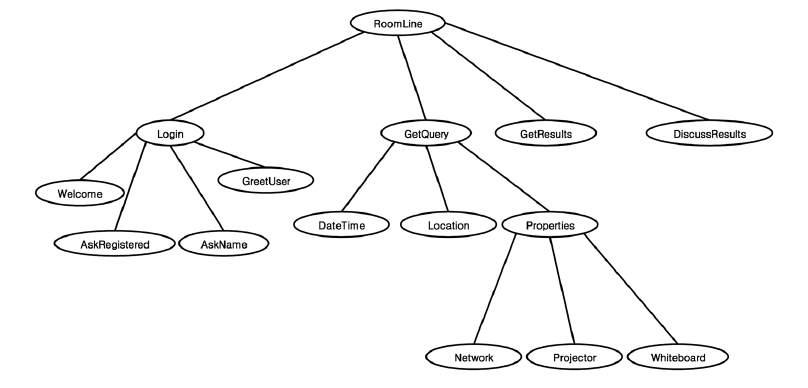
\includegraphics[width=12cm]{figures/knowledgeDM.png}
\caption{基于RavenClaw框架的RoomLine对话管理策略树}
\label{fig:knowledgeDM}
\end{figure}


\item 数据驱动的对话管理

最近几年,对话管理的研究趋势逐步转向数据驱动的方法,即通过语料库来训练相关对话结构和知识库。虽然这种数据驱动的方法需要消耗很大的时间和人力进行语料库标注,但是对话管理模型的训练几乎不需人工干涉,而且在可移植性方面,如果需要在其他领域建立一个对话系统,也只需要重新训练新的语料库,与基于知识的对话管理相比,这显然是更简便的方法。

这些优势驱动了使用无监督强化学习的随机对话建模的发展,如\cite{Levin2000}使用了基于马尔可夫决策过程(MDP)的强化学习算法,\cite{WilliamsYoung2007, Young2013, Williams2013, Kim2015, Henderson2013}使用了基于部分可观测马尔可夫决策过程(POMDP)的强化学习算法来进行对话建模。这些对话管理框架都使用数据驱动的统计机器学习算法,通过强化学习算法来优化系统的奖励或者惩罚函数,允许系统有理论原则性地根据当前的对话状态来动态修改对话策略。此外,基于POMDP的对话管理还能通过支持最优语音识别和自然语言理解结果来评估信念状态(belief state),从而达到纠正语音识别以及自然语言理解模块中出现的错误。对于基于POMDP的对话管理,系统只观测在当前状态下的有关现实世界(在对话系统中指的是语音识别和自然语言理解结果)的不完整的信息,系统必须利用当前对话状态下寻求一种最优策略将当前的信念状态映射到对话管理策略上。因此,基于POMDP的对话管理可以通过维持信念状态(即最优语音识别和自然语言理解结果)分布来实现语音识别和自然语言理解结果的纠错处理,而无需其他特殊方法。同时,有关用户的背景知识(如用户的特长以及情感状态等)也能通过可分解的强化学习模型映射到状态空间中,从而使得对话管理更人性化。

尽管强化学习算法在理论上能解决基于不确定性的推理和决策,从而为对话管理提供了有效的途径,但在实现过程中,基于强化学习的对话系统依然困难重重\cite{Paek2006},首先,对话系统中的状态包含大量语义项和项值、用户意图、理解结果和对话历史的各种可能组合,使得状态空间的规模指数增长\cite{yukai2014},因此使得强化学习的过程计算复杂度巨大,也使得对话控制的精细改进过程变得困难;其次,强化学习得到的最优策略也剥夺了对话系统开发者对对话流程的监督指导权利。\cite{WilliamsYoung2005, Lemon2006, Young2007, Thomson2008, Williams2008b}对这些问题在一定程度上进行了改进。\cite{Lemon2006, Williams2008b}中研究了如何将传统的基于知识的对话管理和基于强化学习的对话管理结合起来构建商务领域的对话管理规则库,在一定程度上给开发人员留下了对对话管理的监督和指导的空间。然而,目前该方法仍在研究中,尚未用到实用性的对话系统中。

数据驱动的对话管理方法还包括使用最大似然估计等有监督的机器学习算法从对话语料库中训练对话模型\cite{Hurtado2005}。为了避免数据稀疏的问题,\cite{Hurtado2005}中采用了对话寄存器来表示对话状态序列用于跟踪对话历史,其中对话寄存器包含用户在整个对话历史中提供的各项信息。

基于实例的对话管理方法也是数据驱动的对话管理中的一个流行的研究方向,具有代表性的系统有\cite{Murao2003, Inui2001, Lee2009c}。该方法假定类似的对话状态会引发类似的回应,因此可以通过匹配对话实例库中的与当前对话状态最相似的对话状态来构建相应的对话模型。目前搜索与当前对话状态最相似的对话实例大多数都使用关键词来检索,对话实例库中的对话实例的表示通常采用语义约束的形式,从而整个对话实例库可以通过语义索引来概括\cite{Lee2009c}。对话管理模块首先将当前的对话状态也表示为语义约束的形式,并试图从对话实例库中找到与之相近的对话实例,如果没有返回结果,系统会放松语义约束后再一次从对话实例库中查找相近的对话实例;如果返回结果不止一个,那么系统会采用启发式算法来计算返回结果中的每一个实例与当前输入的相似度,然后选择相似度最高的返回作为应答。

数据驱动的对话管理的相关研究在近几年来发展可以说是突飞猛进,当下流行的深度机器学习也被用于对话管理领域,通过深度神经网络在大型对话语料库上训练对话模型的研究也取得了比较有前景的实验结果\cite{Shang2015, Sordoni2015b, VinyalsLe2015}。近期的相关研究还包括“端到端”的数据驱动对话管理框架,也就是利用多层次的神经网络对整个对话过程中的每一个组件以及每一个阶段都进行训练,从而得到包含从语音输入到语音输出,以及对话过程中各个阶段的一系列概率模型\cite{Serban2015}。然而,这些数据驱动的方法都严重依赖于足够大的数据集,为了取得有价值的实验结果,动辄需要上千万甚至上亿则对话。

\item 基于混合方法的对话管理

为了克服上述提到的基于知识以及数据驱动的对话管理方法中的各种不足,基于混合方法的对话管理的研究逐渐发展起来。

传统的基于强化学习的对话管理方法需要通过用户和系统的反复交互来学习一个好的对话策略,而且目前的强化学习算法的泛化能力很弱,往往需要通过大量人力去和系统交互或者庞大规模的对话语料库去归纳一个很小语境条件下的对话策略。为了解决该问题,\cite{Pietquin2006, Schatzmann2007}中引入了用户模拟器的技术,也就是说,通过用户模拟器来代替人和对话管理器进行交互。根据有限的真实语料概括学习得到特定的用户模型,用户模拟器可产生大量的模拟对话。除此之外,\cit{Henderson2008}中还提出了将强化学习和有监督学习结合起来并在有限固定的对话语料库上学习和优化对话策略的混合方法,有监督学习的引入在一定程度降低了传统强化学习方法中对巨大对话语料库的需求程度。在该方法中,强化学习用于优化对话策略中对话奖惩的度量,而有监督学习用于指导对学习到的对话策略状态空间的剪枝,从而得到更高效有用的状态空间。

在传统的POMDP算法中,优化过程可以在任何时刻选择任意的行为,因此,没有简洁易操作的方式引入一些领域相关的常识性知识来约束和指导优化过程。例如,一个医疗相关的对话系统不应该在问病人症状之前就提供用药建议,然而,传统的POMDP算法却不存在直接的方法将该常识引入到优化过程中。近年来,也有相关研究提出来改进该问题,如\cite{Lemmon2006, Williams2008b}中提出了在POMDP框架中基于传统规则来约束策略状态中的可能对话行为的集合,这样通过传统规则来对状态空间中的一些不合理的行为进行剪枝,不但加速了强化学习的优化过程,也使优化过程往更可靠的方向进行。

目前,传统的基于实例的对话管理方法应用在实用口语对话系统中还存在很多关键问题,比如先验知识的缺乏,语音识别的错误,以及语义解析的不确定性等。针对这些问题,\cite{Lee2009b}中提出了将对话实例与先验知识同时用在基于实例的对话管理中,从而提高系统的鲁棒性。该方法使用了基于议程的模型,将先验知识表示为议程图,并作为对话管理的子任务流之一来对领域相关的对话控制进行编码。这些先验知识不仅被用于预测系统的下一个对话行为,还通过议程图来跟踪对话状态,以便于处理一些话题焦点转移的意外情况。另外,该方法还通过在话语层次和语篇层次上的打分作为启发,来对当前对话状态下的N-best的对话行为假设进行重排。

基于混合方法的对话管理的最新研究趋势还包括在强化学习模型中引入概率规则的概念,\cite{Lison2015}中将概率规则定义为逻辑条件和概率事件之间的结构映射,并作为高层次的模板用于概率图模型中,其中可能包含未知参数,其值可以通过数据进行贝叶斯推断来估计得出。由于使用了逻辑的抽象化,这些概率规则可以对数据驱动的基于POMDP的对话管理中使用的概率模型进行编码成更紧凑更可读的形式。在理想情况下他们需要较少的参数估计,因此,与典型的基于POMDP的对话管理方法相比,要求较少的训练数据,也允许开发者在对话管理过程中使用人工编写的对话控制规则。然而,该方法还未成熟和完善,其实用价值在很大程度上还有待考察。

\end{enumerate}

在这些繁多的对话管理研究技术中,本文提出的方法更接近于现有技术中的通用对话建模技术,以及最新的在对话管理中引入概率规则的相关研究。然而,与这些研究又不同,本文由系统的动机出发,结合言语行为以及其他的交际行为与这些动机之间的关系来构建一个相当复杂的对话管理模型。此外,由于使用了基于概率逻辑规则的知识表示方法,本文的认知对话管理框架也能通过观测数据来进行对话模式的自适应。因此,本文的方法可以被认为是基于混合方法的对话管理。
从长远角度来看,本文提出的对话管理框架将实现以通过观测数据来进行经验概率分析为主的对话控制,不过目前,我们的研究集中于将其内置的通用对话建模将作为对话行为控制的主导。


%%%%%%%%%%%%%%%%%%%%%%%%%%%%%%%%%%%%%%%%%%%%%%%%%%%%%%%%%%%%%%%
\subsection{自然语言理解、生成研究综述}{Overview of Natural Language Understanding and Generation}
%%%%%%%%%%%%%%%%%%%%%%%%%%%%%%%%%%%%%%%%%%%%%%%%%%%%%%%%%%%%%%%

智能对话系统的研究、开发和使用都离不开自然语言理解和自然语言生成的支持,因此本小节将分别对自然语言理解和自然语言生成方面的现有研究技术以及存在的问题等进行简要的回顾。

\begin{enumerate}

\item{自然语言理解}

自然语言理解是自然语言处理(NLP)的分支领域,它是通过使用软件来理解自然语言的意义(语音,或者本文更关注的“文本”)。自然语言理解主要是将自然语言转换成抽象的语义形式,以获取语言的含义;或者是转换为某种响应(例如对某个问题的回答),以说明其理解了语言的含义。

在20世纪80年代之前,自然语言理解的方法通常是基于人工编写的复杂规则。紧随着机器学习技术的发展,基于统计的自然语言理解方法也开始兴起\cite{Tan1992}。乔姆斯基的形式语法理论以及摩尔定律使得通过语料库来进行统计学习的自然语言理解技术成为可能\cite{Gupta2014}。近些年来,越来越多的相关研究投入到无监督学习或者半监督学习方法上,这些技术能使自然语言理解不那么依靠需要大量人力获得的人工标注的语料库。一般来说,与有监督学习相比,无监督学习或者半监督学习的难度相当大\cite{Gupta2014}。

在目前主流的智能对话系统中,自然语言理解模块通常通过以下流程逐步完成:词法分析、句法分析、语义关系抽取、语义理解。词法分析主要是将字符序列转换为标记序列的过程,并非本文的研究内容,因此这里从其他几方面来介绍各流程的研究现状。


\begin{description}
\item[(1)]{句法分析}
通常自然语言理解是通过对句子的某些,或全部句法法进行分析来完成的。大量的形式化体系和算法通过特定的语法体系对句子的句法结构进行解析。大体来说,主流的句法分析包括“依存句法分析” \cite{Eisner1996a, Eisner1996b, Yamada2003} 以及 “短语结构句法分析” \cite{Chomsky1957, Pollard1994}。短语结构句法分析依据短语结构文法\cite{Thompson1981, Charniak1997, Makino1998, Charniak2006},首先对句子进行短语分析,然后指出单词和短语之间的关系,以及短语之间的关系;而依存句法分析依据依存文法\cite{Tesniere1959, Melchunk1988},仅仅在句子中的单词之间标注(有标记的)连接关系。依存句法分析是我们要在本文中探讨的语法类型。


这里的“依存”是指语言单位(如单词)由有向链接相互联系在一起。一般来说,在依存语法中,(限定)动词被视为句子或子句结构的中心,其它所有句法单位(单词)是直接或间接地与动词通过有向链接相连。这种有向链接被称为“依存”。句子结构是由一个词(中心词)与它的依存词之间的关系而决定的。


“依存”关系是一对一的对应关系:对于句子中的每个元素(例如:单词或语素)来说,实际上句子中都有一个与其相对应的节点。这种一对一的对应关系决定了“依存语法”就是单词(或语素)的语法。所有的句子都有元素和将元素组成结构的依存关系,这种情况应该与短语结构语法的“成分关系”进行比较,“成分关系”是一对一,或一对多的对应关系,也就是说,对于句子中的每个元素来说,有一个或多个与其对应的节点。这种不同带来的结果是:相比短语结构,依存结构非常紧凑,因为它往往包含很多小的节点。从计算机处理的角度来说,这种简洁的结构是有益的。


\item[(2)]{关系抽取}
自然语言理解中的一个重要方向是{\bf 关系抽取}。在NLP领域中,关系抽取已成为一个重要的研究方向,一方面是因为它的实际应用价值,另一方面因为它被看做是语义分析的一部分,而且是目前的技术相对容易实现的那部分。到目前为止,吸引最多注意力的关系抽取是命名实体之间的关系识别,例如:“个人从属关系”和“组织地址关系”。

一般来说,关系可以由一个元组的形式来定义的,$t = (e_1, e_2, ...,e_n)$。在这里,$e_i$ 是文本中预定义关系$r$ 的实体。大多数关系抽取系统主要关注二元关系的抽取。例如 :

\begin{verbatim}
位于(厦门,中国)
father-of(Richard Li, Li Ka-Shing)
\end{verbatim}

抽取“高阶关系”也非常有意义。例如这个句子:"At codons 12, the occurence of point mutations from G to T were observed'' (“在密码子12,观察到从G到T的点突变”)。句子中出现了一个4进制生物医学关系,可以描述为:

\begin{verbatim}
point mutation(codon, 12, G, T)
\end{verbatim}

目前人们普遍视“关系抽取”为一个有监督分类问题,它从一个语料库开始(语料库中包含由人类标记的相关语义关系),然后利用统计方法来对标记的关系建模,并学习出适合应用于其它文本的统计模型。

目前,关系抽取系统的主要限制在句子层面上运用。事实上,关系可能跨越句子,甚至贯穿不同的文件。然而,解决这一问题需要一定的常识和非常灵活的知识表示。本文的研究也无法直接解决这一问题,但我们相信:通过将句子意义映射为通用的知识表示,我们已经奠定了解决问题的基础。在这种知识表示中,跨句或跨文本的通用联系和推理是可以被实现的。

\item[(3)]{流结构语法}


将流结构语法(FCG)与本文使用的语言形式化体系进行比较分析是很有意义的。在FCG中,一句话语的信息是以语义和句法结构组织在一起的。语义结构是对“话语意思”的分解,它含有特定语言的语义分类,例如:“put”事项被归类为“起因-移动-位置”类事项,包括一个施事者(agent)、一个受事者(patient)和一个位置(location)。句法结构是将话语形式分解为成分和词素,还包含附加的句法分类,比如:句法特征(例如:数量和性别)、词序限制等。


从理论上来说,FCG是基于一种程序性语义的方法,在这个意义上,话语的意思是听话人假定要执行的程序,因此,概念化便是一个规划过程(规划该程序),而解析便是对该程序的执行过程。
FCG中,有关配对句法和语义结构的例子(短语“the ball”),请见图 \ref{fig:fcg1} and \ref{fig:fcg2}。

\begin{figure}[htb]
\centering
\includegraphics[width=12cm]{figures/fcg1.png}
\caption{ FCG中对短语“the ball”的句法及语义表示结构}
\label{fig:fcg1}
\end{figure}

\begin{figure}[htb]
\centering
\includegraphics[width=12cm]{figures/fcg2.png}
\caption{ FCG中对短语“the ball”的语义表示的列表形式}
\label{fig:fcg2}
\end{figure}


所有的FCG规则都是双向的。通常在产生过程中,所要表达的语义内容是与语义结构相统一的,有可能产生一组绑定。如果成功了,绑定会与语义结构相融合。这种融合可以理解为“部分统一”,但它利用结构中那些遗漏部分扩展了结构。在句法分析过程中,被分析的句子与句法结构是统一的,同时,结果中的某些部分被添加到语义结构中。
\end{description}

本文所使用的形式化体系在概念上有些类似FCG。 此外,我们有配对句法和语义结构,而且还进行双向处理。在第\ref{chap:comprehension}章中,我们将论述链语法,它将句子转换成句法结构,以及RelEx和RelEx2Logic模块,它们将句法结构转换成语义结构。在第 \ref{chap:generation}章中,我们将阐述另一个方向的Microplanner 和SuReal模块,也就是将语义结构转换成句法结构,再生成句子。本文研究的平台OpenCog中的模式匹配器(Pattern Matcher)在使用这些句法和语义结构时,也将这些结构视为有效的程序,同样实现了“程序化语义”。但我们的形式化体系与FCG的着重点不同。FCG主要是用作探索问题的理论工具,而本文的研究更侧重用于真实世界的实际应用。

\item{自然语言生成}{Natural Language Generation}
XXXX



\cite{Wen2015}

In the past decade, significant progress has been made in applying statistical methods to automate the speech understanding and dialogue management components of an SDS, including making them more easily extensible
to other application domains (Young et al., 2013; Gasiˇc et al., 2014; Henderson et al.,2014). However, due to the difficulty of collecting
semantically-annotated corpora, the use of data-driven NLG for SDS remains relatively unexplored and rule-based generation remains the
norm for most systems (Cheyer and Guzzoni,
2007; Mirkovic and Cavedon, 2011).

在过去的十年中,显著的进步已经在应用统计方法来自动的SDS的言语理解与对话管理部件制成,包括使他们更容易扩展
其他应用领域。然而,由于回收的难度
语义标注语料,进行SDS采用数据驱动的前起落架保持相对未开发的和基于规则的产生仍然是
规范对于大多数系统

随着统计机器学习技术的不断成熟,近十几年来,针对对话系统的自然语言理解研究已经有了显著的进步


The goal of the NLG component of an SDS is
to map an abstract dialogue act consisting of an
act type and a set of attribute-value pairs1
into  an appropriate surface text (see Table 1 below for some examples). An early example of a statistical
NLG system is HALOGEN by Langkilde
and Knight (1998) which uses an n-gram language
model (LM) to rerank a set of candidates generated
by a handcrafted generator. In order to reduce
the amount of handcrafting and make the
approach more useful in SDS, Oh and Rudnicky
(2000) replaced the handcrafted generator with a
set of word-based n-gram LM-based generators,
one for each dialogue type and then reranked the
generator outputs using a set of rules to produce
the final response. Although Oh and Rudnicky
(2000)’s approach limits the amount of handcrafting
to a small set of post-processing rules, their
system incurs a large computational cost in the
over-generation phase and it is difficult to ensure
that all of the required semantics are covered
by the selected output. More recently, a
phrase-based NLG system called BAGEL trained
from utterances aligned with coarse-grained semantic
concepts has been described (Mairesse et
al., 2010; Mairesse and Young, 2014). By implicitly
modelling paraphrases, Bagel can generate
linguistically varied utterances. However, collecting
semantically-aligned corpora is expensive and
time consuming, which limits Bagel’s scalability
to new domains.

自然语言生成(NLG)是自然语言理解(NLU)的反向过程。总的来说,自然语言生成是从信息的计算表示中自动生成人类(自然的)语言。由于语义知识表示体系的差异化,造成自然语言生成系统的输入多样化,因此不同的自然语言生成系统所包含的组块一般都不尽相同。概括地说,自然语言生成系统可以表示为解决下列两项任务:

\begin{itemize}
\item What should I say?(我应该说什么?)
\item How should I say it?(我应该怎么说?)
\end{itemize}

为了解决这些问题,自然语言生成系统可能涉及许多相互关联的规划模块,如:
\begin{itemize}
\item 确定要表达的信息
\item 构建语篇规划
\item 将信息块转换为语篇单位
\item 选择适当的短语和单词
\item 输出正确的语法
\end{itemize}

将这个流程分解为阶段的方法如下:
\begin{description}

\item [1)] 宏观规划

宏观规划涉及选择和组织内容。它输入的是一个或多个沟通目标:解释、描述,或提问;引起听众的某种行动或思考等。宏观规划输出的是一种知识架构,这个架构不一定是语言的属性,而是体现智能体所要沟通的信息。除了一般性内容,这种知识架构可能包含一些与沟通过程有关的信息,例如:不同的知识块应该以什么样的顺序来传达。

目前宏观规划的研究主要基于一些语篇结构层次上特定的理论体系,例如:修辞结构理论\cite{Mann1987}。在本文所介绍的研究中,我们采用了基于动机认知模型Psi的宏观规划,该模型的构建非常符合人类的心理特征。

\item [2)] 微观规划

微观规划则运用知识架构,并将它们分为句块。微观规划必须处理多种语言问题,例如:

\begin{itemize}
\item 句子范围:是否可以将两片叶子接在一起,怎样接在一起。(“我今天饿了。我去了 Burger King。” VS “我今天饿了,所以我去了Burger King。”)
\item 代词化
\item 聚合:删除重复内容。(“抽烟对你不好。抽烟会缩短你的寿命。抽烟让你口气不佳” VS “抽烟对你不好、缩短你的寿命,而且让你口气不佳”)
\item 主题化
\item 主题排序
\end{itemize}

到目前为止,我们的大多数微观规划都是为特定的应用而专门制定的。有一个名为SPUD\cite{Stone 1997}的多用途微观规划框架,它利用的是一个基于逻辑的规划流程形式。尽管在细节上有所不同(原来的SPUD是基于树-邻近语法),但我们所描述的微观规划在概念上受到了SPUD的很大影响。

\item [3)] 表层生成

最后,“表面生成”涉及的是文本表层的生成,例如:把知识结构转换为句子。经典的表层生成器,例如FUF/SURGE\cite{Elhadad1992}和 Penman/KPML\cite{Matthiessen1991},都是以深层语言学理论为基础的。其他知名的系统,例如Nitrogen\cite{Langkilde1998}则采用的是统计法。所有基于规则的方法和统计法现在仍然流行。

\end{description}

一般来说,与自然语言理解相比,自然语言生成技术要落后得多。目前的实用系统往往比较专业化,而且很粗糙。概念比较先进的系统,如FCG,尚未经过广泛地实践测试。正如第\ref{chap:generation}章中所介绍的,我们在这一领域的研究代表了“基于规则的方法”和“统计法”的融合。我们认为这种融合非常有前景,但还没有精细化,也没有经过系统性评估。
\end{enumerate}

%%%%%%%%%%%%%%%%%%%%%%%%%%%%%%%%%%%%%%%%%%%%%%%%%%%%%%%%%%%%%%%
\subsection{言语行为理论及相关研究综述}{Overview of Speech Act Theory and related research}
\label{sec:speechAct}
%%%%%%%%%%%%%%%%%%%%%%%%%%%%%%%%%%%%%%%%%%%%%%%%%%%%%%%%%%%%%%%

我们认为,分析和管理对话系统需要产生的各类话语的一个有效方法是:使用由Austin\cite{Austin2005}提出,Searle\cite{Searle1969} 改进的言语行为理论(Speech Act Theory)。本文将要阐述的智能对话研究中正采用了此方法,且在研究过程中,我们发现这个理论是极其有用且方便使用的。我们在这一节先回顾言语行为理论的基本观点,并介绍一些言语行为理论在对话方面的相关研究以及更细致具体的分类体系。

言语行为理论是语言学和语用学等研究中的一个重要理论。言语行为理论的核心概念是:强调语言的意向功能,认为说话者在说话的同时是在实施某种行为。因此,根据言语行为的观点,分析说话者的语言行为的过程,也就是说话者分析为了实现某个特定目标而采用的一系列的言语行为的过程。

言语行为理论探讨那些可以通过言语来表现的行为类型。Austin\cite{Austin2005}将言语行为分为以下几种:

\begin{itemize}
\item {\bf 言内行为(Locutionary Act)}:话语的外在表现形式,即:话语本身的字面意义。
\item {\bf 言外行为(Illocutionary Act)}:话语的“言外之力”,即:说话者对受话者的影响。
\item {\bf 言后行为(Perlocutionary Act)}:话语达到的实际效果,即:话语所导致的行为,如说服、劝说、吓唬、启发、激励,或者让受话者去做某件事,或者让受话者意识到什么,不论是有意还是无意的。
\end{itemize}

Searle对Austin提出的言语行为理论做了深入的研究和探讨。在Searle\cite{Searle1969}看来,言语行为有时仅仅指的是言外行为。他认为,说话人通过他们的言语只能获得5类言外之力,它们分别是:

\begin{itemize}
\item 断言类:说话人自己承诺事情是真的。The sky is blue. (天是蓝色的。)
\item 指令类:说话人试图让受话人做某事。Clean your room! (打扫你的房间!)
\item 承诺类:说话人对未来的行为做出承诺。I will do it. (我将会做这件事。)
\item 表达类:说话者表达了某些心理状态。I’m Sorry. (对不起。)。
\item 声明类:说话人带来了不同的状况。The meeting is adjourned.(这个会议休会了。)
\end{itemize}

受这个本体论的启发,Twitchell 和 Nunamake在他们2004年的论文(标题为:言语行为归档:分析持续谈话和其参与者的概率统计法。\cite{Twitchell2004})中提出了更加精细的“42种言语行为”本体论,叫做SWBD-DAMSL (DAMSL = Dialogue Act Markup in Several Layers)。尽管有少量不符合Searle的观点,并被分类为“其它”,但几乎他们所有的42种言语行为类型都能够被映射到Searle的5个高级类别之一。图\ref{fig:DAMSL}和\ref{fig:Searle}描述了这42种行为和它们与Searle分类之间的关系。我们已经利用了这个Searle解析法,它给我们正在进行的自然语言对话研究带来了灵感。

\begin{figure}[htb]
\centering
\includegraphics[width=12cm]{figures/DAMSL.png}
\caption{SWBD-DAMSL中使用的42种言语行为}
\label{fig:DAMSL}
\end{figure}

\begin{figure}[htb]
\centering
\includegraphics[width=12cm]{figures/Searle.png}
\caption{ 42种SWBD-DAMSL言语行为类型与Searle的言语行为类型的关联}
\label{fig:Searle}
\end{figure}


总之,言语行为理论为对话管理和对话控制提供了一个新的思路,也就是将对话的话语看成是一种行为,这样不仅能通过对不同言语行为的定义来猜测说话人的意图,还能将对话行为看成和其他非语言的行为类似。不难看出,它不仅给对话管理和对话控制提供更多可行的用于非语言的行为控制机制,也同时能将对话与智能体的其他行为有效结合起来,从而完成更智能更人性化的对话。

%%%%%%%%%%%%%%%%%%%%%%%%%%%%%%%%%%%%%%%%%%%%%%%%%%%%%%%%%%%%%%%
\section{存在的问题}{Omissions of Present Research}
%%%%%%%%%%%%%%%%%%%%%%%%%%%%%%%%%%%%%%%%%%%%%%%%%%%%%%%%%%%%%%%

XXXXXX需要修改:按照上面的顺序来介绍每一领域的相关研究出现的问题,即知识表示逻辑推理、言语行为理论的应用、对话系统、自然语言理解和生成。

虽然上述工作已经取得了重要成果,但是从一个更广阔的视野来看,仍然还有很多未完成的工作,其中有许多也是我们目前正在研究和开发的课题。

首先必须强调的是,截止到我们目前所做工作为止,语言理解和生成的许多关键方面一直未被关注,甚至完全被忽略。如以下几个例子:
\begin{itemize}
\item 形态。链语法分析器,作为上述理解系统的初始阶段,最近已扩展到在语素及文字水平进行句法分析;但我们还没有将这项工作纳入到我们自己的工作中。
\item 语用。我们能够按照他们的实际能力对语句生成逻辑表达式进行分析,但是我们并未执行语用方面的分析。
\item 消歧。我们已在OpenCog框架中实现了一个简单词义消歧系统,但还没有集成到本文的工作中。
\item 名词的回指消解。在我们的理解系统内,人称代词的指代消解已通过各种启发式算法实现,但名词的回指却被忽略。
\end{itemize}

目前我们工作的一部分是指出整体框架中的这些缺陷。然而,我们相信即使给出这些疏漏,我们所做的工作也足够为以上三个假设提供合理的证据支持。展示处理上述现象能力必然有助于compelling system,但是对于验证本方法和三个假设的有效性并不必要。

本文工作的其中一个目标就是构建一个具有一定智力水平的智能会话系统。为了实现这样的智能会话系统,本文也开发了涉及自然语言理解、生成和推理等的相关模块。但本文的工作并不仅仅包括自然语言理解、生成和推理本身,例如还包括下面几个方面:
\begin{itemize}
\item 来自语言的逻辑表达和来自其他信息渠道的逻辑表达的有效整合,这些其他信息渠道可以是机器人或虚拟世界里的涉身知识,也可以是限定领域的标注语料库
\item “对话控制程序”的实现,该对话控制程序从一个动机驱动的系统中获取相关信号,然后结合系统当前的动机、最近的语言输入以及当前的系统知识等相关语境知识来选择相应的语言应答。
\item 额外的推理控制机制,使得智能体在被不相关或者不完全相关的信息来源打断后,仍能进行相对复杂的推理,从而给出相关的应答。
\end{itemize}

这些模块的当前现状将在第 \ref{chap:inference}和\ref{chap:dialogue} 章介绍。这些工作目前还无法在所有的语言现象中得到了验证,还有待进一步深入研究。然而, 在理解、生成和推理等方面,明确的研究方向和相关工具的实现,无疑为以后的研究奠定了结实的基础和提供了一个便捷的研究平台。我们提出三个核心假设的主要原因,是因为它们提供了一种有效的方法,能够借助自然语言理解、生成和语义推理等子系统,来搭建一个大型的智能对话体系结构。

%%%%%%%%%%%%%%%%%%%%%%%%%%%%%%%%%%%%%%%%%%%%%%%%%%%%%%%%%%%%%%%
\section{研究目标和内容}{Goals and Contributions}
%%%%%%%%%%%%%%%%%%%%%%%%%%%%%%%%%%%%%%%%%%%%%%%%%%%%%%%%%%%%%%%
提出创新点

%%%%%%%%%%%%%%%%%%%%%%%%%%%%%%%%%%%%%%%%%%%%%%%%%%%%%%%%%%%%%%%
\section{论文的组织结构}{Outline}
%%%%%%%%%%%%%%%%%%%%%%%%%%%%%%%%%%%%%%%%%%%%%%%%%%%%%%%%%%%%%%%


